\documentclass[aspectratio=169]{beamer}

\usepackage{amsmath}
\usepackage{amssymb}
\usepackage{graphicx}
\usepackage{multirow}

\usepackage{lipsum}% http://ctan.org/pkg/lipsum
\usepackage[utf8]{inputenc}
\usepackage[english]{babel}
\usepackage{amsmath}
\usepackage{amsfonts}
\usepackage{amssymb}
\usepackage{graphicx}

\usepackage{fancyhdr}
\usepackage{hyperref}
%\usepackage{siunitx}
\usepackage{booktabs}
\usepackage{xcolor}
\usepackage{afterpage}
\usepackage{physics}
\usepackage{siunitx}[=v2]
\usepackage{nicefrac}
\usepackage{blindtext}

\usepackage{cuted}
\usepackage{flushend}
\usepackage{subcaption}

%\colorlet{rorange}{orange!70!black}
\definecolor{rorange}{RGB}{223,107,85}
\definecolor{rblue}{RGB}{114,177,236}

\usepackage[T1]{fontenc}
%\usepackage[onehalfspacing]{setspace}
%\usepackage[superscript,biblabel]{cite}
%\makeatletter \renewcommand{\@citess}[1]{\textsuperscript{\,[#1]}} \makeatother

% ##################################################
% BIBLIOGRAPHY
% ##################################################
\usepackage{csquotes}
\usepackage[backend=biber,bibstyle=ieee, citestyle=numeric-comp]{biblatex}
\addbibresource{./BA.bib}
\addbibresource{SHIP-proposal.bib}
\addbibresource{ZINTH.bib}
\addbibresource{SPECTRAL-SEMICONDUCTOR.bib}
\setlength\bibitemsep{.5\baselineskip}
\setcounter{biburlnumpenalty}{9000} % break URLs on numbers
\setcounter{biburllcpenalty}{9000}  % break URLs on lower case letters
\setcounter{biburlucpenalty}{9000}  % break URLs on upper case letters



\usetheme{Darmstadt}
\usecolortheme{dove}

\DeclareSIUnit\eVperc{\eV\per\clight\squared}
\DeclareSIUnit\clight{\text{\ensuremath{c}}}

%\usepackage{caption}
%\captionsetup[figure]{font=footnotesize}
\setbeamertemplate{caption}{\insertcaption} 
\setbeamerfont{caption}{family=\sffamily, size={\fontsize{6}{6}}}
\setbeamercolor{caption}{fg=gray}
\setbeamercolor{caption name}{fg=gray}

\title{\textbf{Study of the position-dependent detector response of a liquid scintillator detector instrumented with WOMs and SiPMs using cosmic muons}}
\author{Andrea Ernst}
\institute{Bachelor's Thesis, Department of Physics, Humboldt-Universität zu Berlin}
\date{11. November 2021}


\setbeamertemplate{itemize items}{--}
\setbeamercolor{itemize item}{fg=rorange}
\setbeamertemplate{enumerate items}[default]
\setbeamercolor{enumerate items}{fg=rorange}

\captionsetup{labelformat=empty,labelsep=none}

\setbeamertemplate{section in toc}{%
	{\color{rorange}\inserttocsectionnumber.}~\inserttocsection}
\setbeamercolor{subsection in toc}{bg=white,fg=structure}
\setbeamertemplate{subsection in toc}{%
	\hspace{1.2em}{\color{rorange}\rule[0.3ex]{3pt}{3pt}}~\inserttocsubsection\par}

\setbeamertemplate{bibliography item}[text]
\setbeamertemplate{bibliography entry article}{}
\setbeamertemplate{bibliography entry title}{}
\setbeamertemplate{bibliography entry location}{}
\setbeamertemplate{bibliography entry note}{}

\setbeamerfont{bibliography item}{size={\fontsize{6}{6}}}
\setbeamerfont{bibliography entry author}{size={\fontsize{6}{6}}}
\setbeamerfont{bibliography entry title}{size={\fontsize{6}{6}}}
\setbeamerfont{bibliography entry location}{size={\fontsize{6}{6}}}
\setbeamerfont{bibliography entry note}{size={\fontsize{6}{6}}}

\setbeamertemplate{footline}{%
	\leavevmode%
	\hbox{%
		\begin{beamercolorbox}[wd=.25\paperwidth,ht=2.25ex,dp=1ex,center]{author in head/foot}%
			\usebeamerfont{author in head/foot}{\color{gray}\insertshortauthor~~}%(\insertshortinstitute)
		\end{beamercolorbox}%
		\begin{beamercolorbox}[wd=.65\paperwidth,ht=2.25ex,dp=1ex,right]{title in head/foot}%
			\usebeamerfont{title in head/foot} 
			\color{gray}\insertframenumber/\inserttotalframenumber{} \hspace*{2ex}
		\end{beamercolorbox}%
		%\begin{beamercolorbox}[wd=.25\paperwidth,ht=2.25ex,dp=1ex,right]{date in head/foot}%
		%\insertframenumber{} \hspace*{2ex}
		%\end{beamercolorbox}
	}%
	\vskip0pt%
}

\begin{document}
	
	\begin{frame}[plain]
		\maketitle
	\end{frame}
	
	
	\begin{frame}{Overview}
		\tableofcontents
	\end{frame}
	
	%------- SHiP -------%
	\section{SHiP}
	
	
	
	
	
	\begin{frame}{Search for Hidden Particles (SHiP)}
		
		\begin{figure}
			\centering
			\includegraphics[width=.8\textwidth]{pictures/ship-facility.pdf}
			\caption{Cr.: SHiP Collaboration \cite{SHIP-DESIGN-2019}.}
		\end{figure}
		
		
		
		\begin{itemize}
			\item 'intensity frontier' experiment to be built at CERN SPS
			\item \SI{400}{\giga\electronvolt} proton beam-dump
			\item looking for long-lived exotic particles, $m < \order{10}\SI{}{\giga\eVperc}$
			 
		\end{itemize}
	\end{frame}


	\begin{frame}{}
	
	\begin{figure}
		\centering
		\includegraphics[width=.8\textwidth]{pictures/ship-facility.pdf}
		\caption{Cr.: SHiP Collaboration \cite{SHIP-DESIGN-2019}.}
	\end{figure}
	
	
	
	\begin{itemize}
		\item target $\rightarrow$ muon shield $\rightarrow$ Scattering and Neutrino Detector
		\item decay volume $\rightarrow$ Hidden Sector decay spectrometer
		\item intensity frontier $\Rightarrow$ need precise background suppression 
		
	\end{itemize}
\end{frame}



	
	\begin{frame}{Surround Background Tagger (SBT)}
		
		\begin{figure}
			\centering
			
\includegraphics[width=.7\textwidth]{pictures/decay_volume.pdf}
			\caption{Cr.: Miano et al \cite{MIANO}.}
		\end{figure}
	\vspace{-.5cm}
		\begin{itemize}
			\item structure surrounds evacuated decay vessel
			\item requirements: 
				\begin{itemize}
					\item full coverage of surrounding area
					\item high detection efficiency of charged particles (muons)
				\end{itemize}
			$\Rightarrow$ liquid scintillator (LS) LAB + PPO chosen
			\item SBT made up of $\order{2000}$ detector 'cells'
			
		\end{itemize}
		
	\end{frame}
	
	
	
	%------- SBT cell prototype -------%
	\section{SBT Cell Prototype}
	
	
	
	
	%------- WOM -------%
	
	\begin{frame}{Wavelength-shifting Optical Module (WOM)}
		\begin{columns}
			\begin{column}{0.5\textwidth}
				\begin{figure}
					\centering
					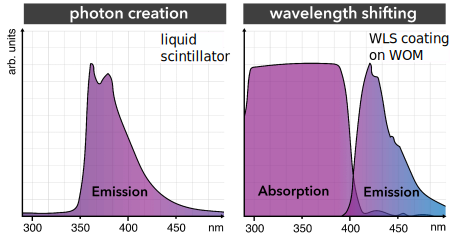
\includegraphics[width=\textwidth]{pictures/absorption-emission.png}
					\caption{Adapted from \cite{ZIMMERMANN}.}
				\end{figure}
				
			\end{column}
			
			\begin{column}{0.5\textwidth}
				\begin{itemize}
					\item emission maximum of LS around 350 to \SI{400}{\nano\meter} $\rightarrow$ not easily detectable
					\item use wavelength-shifting paint on WOM $\rightarrow$ paint absorbs LS photons, re-emits in visible spectrum
				\end{itemize}
				
			\end{column}
		\end{columns}
	\end{frame}


	\begin{frame}{Wavelength-shifting Optical Module (WOM)}
		\vspace{-1cm}
		
		\begin{columns}
			
			\begin{column}{0.3\textwidth}
				\begin{itemize}
					\item LS light enters PMMA tube $\rightarrow$ gets wavelength-shifted $\rightarrow$ shifted light travels in tube (total reflection)
					\item pro: high surface area $\rightarrow$ gathers a lot of light from LS
					\item con: path of light to end of tube can be arbitrarily complex
				\end{itemize}
				
			\end{column}
		
		
			\begin{column}{0.7\textwidth}
				\begin{figure}
					\centering
					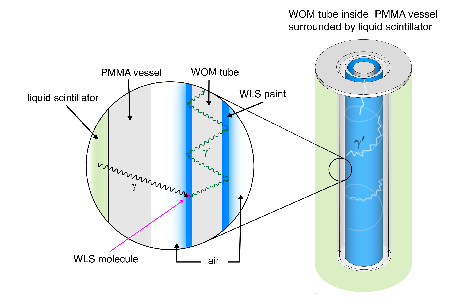
\includegraphics[width=.9\textwidth]{pictures/wom-principle.pdf}
					\caption{Adapted from \cite{ZIMMERMANN}.}
				\end{figure}
				
			\end{column}
		
		\end{columns}


	\end{frame}
	
	\begin{frame}{SBT Cell Prototype}
		\vspace{-1cm}
		\begin{columns}
			
			\begin{column}{0.4\textwidth}
				\begin{figure}
					\centering
					\includegraphics[width=.8\textwidth]{pictures/WOM_Vessel_TB18_top.jpeg}
					\caption{Cr.: DESY.}
				\end{figure}
			\end{column}
			
			
			
			\begin{column}{0.7\textwidth}
				\begin{figure}
					\centering
					\includegraphics[width=.6\textwidth]{pictures/sipm-array.pdf}
				\end{figure}
			
				\begin{itemize}
					\item WOM optically coupled to circular array of 40 SiPMs
					\item SiPMs mounted on PCB, PCB connected to eMUSIC board $\rightarrow$ 40 signals gathered in 8 analog channels
					\item eMUSIC board connected to WaveCatcher (A-to-D converter)
				\end{itemize}
			
			\end{column}
			
			
			
			
			
		\end{columns}
	
	\end{frame}
	
	
	
	
	
	
	\begin{frame}{SBT Cell Prototype}
		\begin{columns}
			
			\begin{column}{0.5\textwidth}
				\begin{itemize}
					\item WOM and LS contained in $\SI{50.4 x 50.4 x 25}{\centi\meter}$ steel box
					\item SiPM array and electronics covered to prevent light leakage
					\item two sets of plastic scintillators + PMTs used to trigger on cosmic muons
				\end{itemize}
			\end{column}
		
			\begin{column}{0.5\textwidth}
					\begin{figure}
						\centering
						\includegraphics[width=\textwidth]{pictures/cosmics-photo.pdf}
					\end{figure}
			\end{column}
			
			
			
			
			
		\end{columns}
	\end{frame}

	\begin{frame}{Position-dependent Detector Response}
		\centering
		
		\includegraphics[width=.8\textwidth]{pictures/cosmics.pdf}
		
		\begin{columns}
			\begin{column}{.5\textwidth}
				\centering
				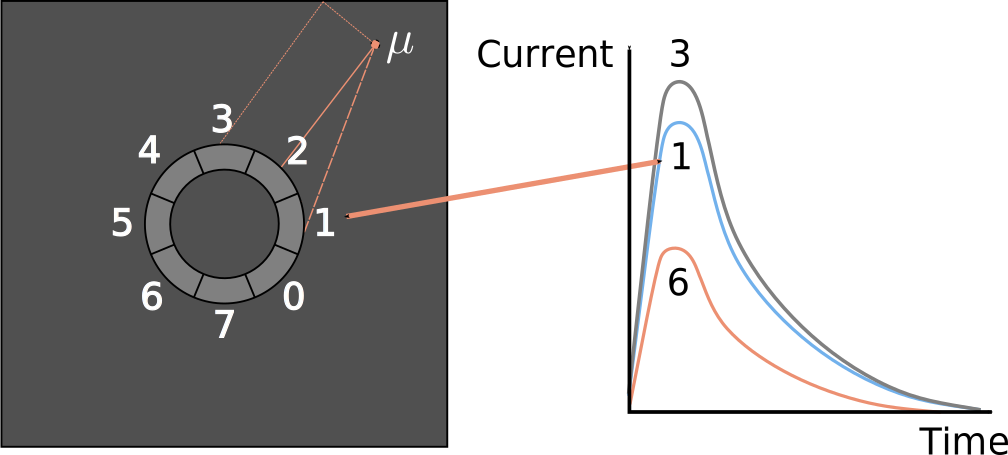
\includegraphics[width=1\textwidth]{pictures/detector-response.pdf}	
			\end{column}
		
			\begin{column}{.5\textwidth}
				\begin{itemize}
					\item muon generates scintillation light in LS box
					\item light gets collected, shifted by WOM $\rightarrow$ travels to SiPM array
					\item goal: study SiPM signal in relation to muon incidence location
				\end{itemize}
			\end{column}
		
		\end{columns}
	
	\end{frame}

	
	
	
	
	%------- CCD vs. TES -------%
	\section{Data Analysis and Results}
	
	\begin{frame}{SiPM Signal}
		\vspace{-1cm}
		\begin{columns}
			\begin{column}{.5\textwidth}
				\centering
				\includegraphics[width=1\textwidth]{pictures/integration-window.pdf}
			
				Light yield:
				\begin{equation*}
					J = \int_{\Delta t} U(t) \,dt
				\end{equation*}
				
			\end{column}
		
			\begin{column}{.5\textwidth}
				\centering
				
				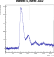
\includegraphics[width=.6\textwidth]{pictures/waveform-sipm.pdf}
				\begin{itemize}
					\item WaveCatcher records \SI{320}{\nano\second} voltage waveform per event and channel group
					\item 'main signal' integrated using RootReader software \cite{ROOTREADER} $\rightarrow$ light yield measure for amount of light collected per channel
				\end{itemize}
			\end{column}
		
		\end{columns}
		
	\end{frame}

	\begin{frame}{Muon Incidence Location}
		\begin{columns}
			\begin{column}{.5\textwidth}
				\centering
				\includegraphics[width=.7\textwidth]{pictures/positional.pdf}
				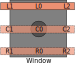
\includegraphics[width=.5\textwidth]{pictures/locations_cosmics.pdf}
			\end{column}
		
		
			\begin{column}{.5\textwidth}
				\begin{itemize}
					\item muon location can be determined using speed of light inside plastic scintillators $c_{PS}$
				\end{itemize}
			\begin{equation*}
				X_{bot} =  \frac{1}{2} \cdot c_{PS} \cdot (t_4 - t_3) = \frac{1}{2} \cdot c_{PS} \cdot \Delta t_{43}
			\end{equation*}
		
			\begin{itemize}
				\item same for $X_{top}$ $\rightarrow$ can filter $\Delta t$ to set location
				\item compare detector signals for 9 positions
			\end{itemize}
		
		
			\end{column}
		\end{columns}

	\end{frame}


	\begin{frame}{Event-dependent Mean Angle $\phi_{ew}$}
		\begin{columns}
			
		
			\begin{column}{.5\textwidth}
				\centering
				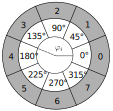
\includegraphics[width=.5\textwidth]{pictures/phi_channel.pdf}
				
				
				\begin{gather}
					\begin{align*}
						x_{i}& = \cos(\varphi_{i}) \cdot J_{i} 
						& y_{i} &= \sin(\varphi_{i}) \cdot J_{i}\\
						X  &= \sum_{i=0}^{7} x_{i}
						& Y &= \sum_{i=0}^{7} y_{i}\\
					\end{align*}
				\end{gather}
			
				
				
			\end{column}
		
			\begin{column}{.5\textwidth}
				\vspace{-1cm}
				\begin{itemize}
					\item assign angle $\varphi_{i}$ to each channel i
					\item average all angles $\varphi_{i}$ weighted by light yield in respective channel $J_i$ $\rightarrow$ use vectorial addition to not introduce false values
					\item convert averaged vector back to polar angle $\phi_{ew}$, project on $\left[-\ang{180},\ang{180}\right]$ interval
				\end{itemize}
%				\vspace{-.1cm}			
				\begin{align*}
					\label{eq:phiew}
					\phi_{ew} = \arctan\qty(\frac{Y}{X})
				\end{align*}
				
			\end{column}
		
		\end{columns}
	\end{frame}
	
	\begin{frame}{Position-dependent Mean angle $\overline{\Phi_{ew}}$}
		\begin{columns}
			\begin{column}{.4\textwidth}
%				\centering
				
				\includegraphics[width=1.1\textwidth]{pictures/phi_ew_R0.pdf}
				
			\end{column}
			\begin{column}{.6\textwidth}
				\centering
%				\includegraphics[width=.9\textwidth]{pictures/phi_ew_R0_shift.pdf}
				\begin{itemize}
					\item sample $\phi_{ew}$ distribution for position R-0
					\item barring shift of mean, similar for all positions except C-0
					\item fit Gaussian to determine position-dependent mean angle $\overline{\Phi_{ew}}$
				\end{itemize}
				
				
			\end{column}
		\end{columns}
	\end{frame}
	
	\begin{frame}{Position-dependent Mean angle $\overline{\Phi_{ew}}$}
		\begin{columns}
			
			\begin{column}{0.4\textwidth}
				\centering
				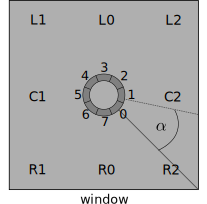
\includegraphics[width=.7\textwidth]{pictures/relative-locations.pdf}
				\begin{itemize}
					\item assign angle $\alpha$ to each muon incidence location
					\item $\alpha \in \left[-\ang{180},\ang{180}\right]$, so that $\alpha = 0$ corresponds to channel 0
				\end{itemize}
			\end{column}
		
			\begin{column}{0.6\textwidth}
				\includegraphics[width=\textwidth]{pictures/phi-ew-std-sep.pdf}
			\end{column}
		
		\end{columns}
	
	
	\end{frame}

	\begin{frame}{Comparison to TestBeam 2019 Results}
		\vspace{-.7cm}
		\begin{columns}
			
			\begin{column}{0.5\textwidth}
				\centering
				\begin{figure}
				\caption{Cr.: Joscha Hanel \cite{HANEL}.}
				\vspace{-.2cm}
				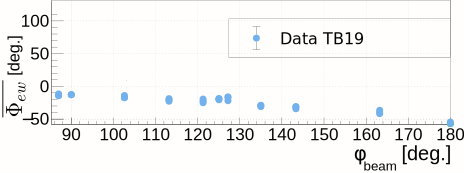
\includegraphics[width=.9\textwidth]{pictures/hanel_phi-ew.pdf}
				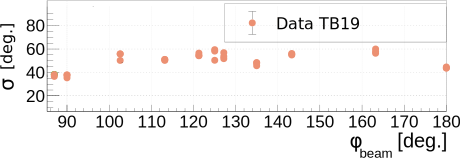
\includegraphics[width=.9\textwidth]{pictures/hanel_phi-std.pdf}
				\end{figure}
			\vspace{-.2cm}
				\begin{itemize}
					\item $\Delta \phi_{beam} = \ang{90} \rightarrow \Delta \overline{\Phi_{ew}} = \ang{45}$
				\end{itemize}
				
			\end{column}
			
			\begin{column}{0.5\textwidth}
				\centering
%				\vspace{-.5cm}
				\includegraphics[width=1.1\textwidth]{pictures/phi-ew-std-sep.pdf}
				
				\begin{itemize}
					\item $\Delta \alpha = \ang{90} \rightarrow \Delta \overline{\Phi_{ew}} = \ang{28}, \ang{74}, \ang{9}, \ang{54}$
				\end{itemize}
			\end{column}
			
		\end{columns}
		\centering
		\vspace{.1cm}
	Standard deviations similar for both, $\overline{\Phi_{ew}}$ overlap with standard deviations
		
	\end{frame}

	\begin{frame}{Central Position C-0}
		\begin{columns}
			\begin{column}{0,5\textwidth}
				\centering
				\begin{itemize}
					\item with ideal optical coupling between WOM and SiPMs, expect uniform $\phi_{ew}$ distribution for C-0 $\rightarrow$ could use this to study coupling in future
				\end{itemize}
			\end{column}
		\begin{column}{0,5\textwidth}
			\begin{figure}
				\includegraphics[width=\textwidth]{pictures/phi-ew-c0-fit.pdf}
			\end{figure}
			
			\end{column}
		\end{columns}
	$\rightarrow$ not uniform! values distributed around ch. 0 \linebreak
	$\rightarrow$ in line with distribution of $\overline{\Phi_{ew}}$ also close to ch. 0 \linebreak
	$\Rightarrow$ optical coupling not ideal
	\end{frame}
	
	
	
	
	% --- Outlook ----
	\section{Summary and Outlook}
	
	\begin{frame}{Summary and Outlook}
		\begin{columns}[t]
			\begin{column}{.5\textwidth}
				\centering
				\textit{can} resolve muon incidence position from SiPM signal to about $\ang{90}$ for many events
%				\vspace*{\fill}
			\end{column}
			\begin{column}{.5\textwidth}
				$\rightarrow$ can \textit{not} determine position of individual event solely from SiPM signal with certainty \linebreak
				$\rightarrow$ need to improve (understanding of) detector
			\end{column}
		\end{columns}
	\vspace{1cm}
	\centering
	Next steps:
		\begin{itemize}
			\item optical coupling between WOM and SiPM array has significant influence on signals \\
			$\rightarrow$ study central position e.g. with external source
			\item make analysis independent of number of detected photons \\
			$\rightarrow$ normalise light yield $\overline{J_i} = \frac{J_i}{\sum_{k=0}^{7} J_k}$
%			\item increase concentration of muons per position \\
%			$\rightarrow$ position determination limited by plastic scintillators' time resolution \\
%			$\rightarrow$ low rate of muons necessitates long measurement runs
		\end{itemize}
	\end{frame}
	
	\section{}
	\begin{frame}
		\vfill
		\vfill
		\vspace*{\fill}
		\begin{flushright}
					Thank you for listening!
		\end{flushright}

		
	\end{frame}
	
	\section{}
	
	%------- References -------%
%	\begin{singlespace}
		\printbibliography
%	\end{singlespace}
	 
	
	
%% backup
\section{}
\begin{frame}{Scintillation Detection}
	
	\begin{columns}
		\begin{column}{0.5\textwidth}
			\begin{itemize}
				\item organic scintillators have delocalised electrons
				\item electron in ground state $S_0$ can absorb photon $\rightarrow$ excitation
				\item excited states $S_{1,2}$ not stable $\rightarrow$ radiationless transitions ($S_2 \rightarrow S_1$), de-excitation via photon emission ($S_1 \rightarrow S_0$) $\rightarrow$ fluorescence
			\end{itemize}
		\end{column}
		
		\begin{column}{0.5\textwidth}
			\begin{figure}
				\centering
				\includegraphics[width=\textwidth]{pictures/jablonski.pdf}
				\caption{Based on \cite{SCINTILLATION-TORRES}.}
			\end{figure}
		\end{column}
	\end{columns}
	
\end{frame}

\begin{frame}{Scintillation Detection}
	
	\begin{columns}
		\begin{column}{0.5\textwidth}
			\begin{itemize}
				\item suppressed secondary process: phosphorescence
				\item fluorescence $\sim \order{1}\SI{}{\nano\second}$
				\item phosphorescence $\sim \order{1}\SI{}{\micro\second}$ \\
				
			\end{itemize}
			$\Rightarrow$ 'efficiency' of scintillator lowered for small time scales
		\end{column}
		
		\begin{column}{0.5\textwidth}
			\begin{figure}
				\centering
				\includegraphics[width=\textwidth]{pictures/jablonski.pdf}
				\caption{Based on \cite{SCINTILLATION-TORRES}.}
			\end{figure}
		\end{column}
	\end{columns}
	
\end{frame}

\begin{frame}
	\begin{figure}
		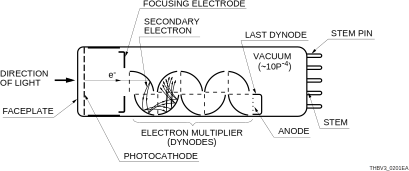
\includegraphics[width=.7\textwidth]{pictures/photomultiplier.pdf}
		\caption{Cr.: Hamamatsu \cite{HAMAMATSU-PMT}.}
	\end{figure}
\begin{itemize}
	\item photoelectrons get multiplied by acceleration and knocking more electrons lose
	\item response time mainly from number of multiplications, acceleration time, transit time to anode
\end{itemize}
\end{frame}


	
	\begin{frame}
		\begin{figure}
			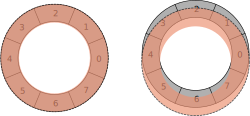
\includegraphics[width=.5\textwidth]{pictures/coverage.pdf}
		\end{figure}
	\begin{itemize}
		\item imperfect coverage of WOM by SiPM array could favour some channels
	\end{itemize}
	\end{frame}
	
	
\end{document}
